\subsection{Exercise 6.1: Graph Transpose}
\textbf{Problem:} The transpose of a directed graph $G = (V,E)$ is the graph $G^T = (V,E^T)$, where $E^T = \{(u,v) \mid (v,u) \in E\}$. Describe efficient algorithms for computing $G^T$ from $G$, for both the adjacency-list and adjacency-matrix representations of $G$. Analyze the running times of your algorithms.

\textbf{Solution:} Let's analyze both representations:

\textbf{1. Adjacency Matrix Representation:}
\begin{itemize}[noitemsep]
    \item Let $|V| = n$. If $M_G$ is the adjacency matrix of $G$, then $M_G^T$ is the adjacency matrix of $G^T$
    \item For a matrix $M$:
        \[ M = \begin{pmatrix}
            m_{11} & m_{12} & \cdots & m_{1n} \\
            m_{21} & m_{22} & \cdots & m_{2n} \\
            \vdots & \vdots & \ddots & \vdots \\
            m_{n1} & m_{n2} & \cdots & m_{nn}
        \end{pmatrix} \]
    \item The transpose matrix is:
        \[ M^T = \begin{pmatrix}
            m_{11} & m_{21} & \cdots & m_{n1} \\
            m_{12} & m_{22} & \cdots & m_{n2} \\
            \vdots & \vdots & \ddots & \vdots \\
            m_{1n} & m_{2n} & \cdots & m_{nn}
        \end{pmatrix} \]
    \item Example:
        \[ M = \begin{pmatrix}
            1 & 2 \\
            3 & 4
        \end{pmatrix}, \quad
        M^T = \begin{pmatrix}
            1 & 3 \\
            2 & 4
        \end{pmatrix} \]
    \item Algorithm:
        \begin{itemize}[noitemsep]
            \item Swap all pairs $(m_{ij}, m_{ji})$ outside main diagonal
            \item Number of swaps: $n^2 - n$ (excluding diagonal)
            \item Time complexity: $\Theta(n^2)$
        \end{itemize}
\end{itemize}

\textbf{2. Adjacency List Representation:}
\begin{itemize}[noitemsep]
    \item Algorithm:
        \begin{enumerate}[noitemsep]
            \item Create new "vertical list" with all vertices $V$ of $G^T$ (same as $G$)
                \begin{itemize}[noitemsep]
                    \item Cost: $\Theta(n)$
                \end{itemize}
            \item For each vertex $v$ in $G$'s adjacency list:
                \begin{itemize}[noitemsep]
                    \item For each vertex $w$ in $v$'s list:
                        \begin{itemize}[noitemsep]
                            \item Add $v$ to $w$'s list in $G^T$
                        \end{itemize}
                \end{itemize}
            \item Total cost: $\Theta(|V| + |E|)$
        \end{enumerate}
\end{itemize}

\textbf{Complexity Analysis:}
\begin{itemize}[noitemsep]
    \item Adjacency Matrix: $\Theta(n^2)$
        \begin{itemize}[noitemsep]
            \item Must process every cell in matrix
            \item Independent of number of edges
        \end{itemize}
    \item Adjacency List: $\Theta(|V| + |E|)$
        \begin{itemize}[noitemsep]
            \item Must process each vertex once
            \item Must process each edge once
            \item More efficient for sparse graphs
        \end{itemize}
\end{itemize}

\textbf{Key Insights:}
\begin{itemize}[noitemsep]
    \item For dense graphs ($|E| \approx |V|^2$), both representations have similar performance
    \item For sparse graphs ($|E| \ll |V|^2$), adjacency list is more efficient
    \item Space complexity matches time complexity for both representations
\end{itemize}

\subsection{Exercise 6.2: Dijkstra's Algorithm with Negative Weights}
\textbf{Problem:} Give a simple example of a directed graph with some negative-weight edges for which Dijkstra's algorithm produces incorrect answers.

\textbf{Solution:} Any directed graph containing a cycle with a negative total weight will cause Dijkstra's algorithm to produce incorrect answers. Here's a simple example:

\begin{figure}[H]
\centering
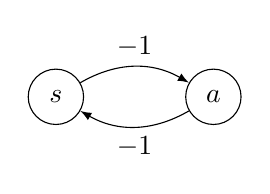
\begin{tikzpicture}[
    vertex/.style={circle,draw,minimum size=20pt,inner sep=0pt},
    >=latex
]
    % Vertices
    \node[vertex] (s) at (0,0) {$s$};
    \node[vertex] (a) at (2,0) {$a$};
    
    % Edges with weights
    \draw[->] (s) to[bend left=30] node[above] {$-1$} (a);
    \draw[->] (a) to[bend left=30] node[below] {$-1$} (s);
\end{tikzpicture}
\caption*{A graph with negative-weight cycle}
\end{figure}

\textbf{Why This Breaks Dijkstra's Algorithm:}
\begin{itemize}[noitemsep]
    \item Dijkstra's algorithm assumes that adding an edge to a path cannot decrease its total weight
    \item In this example:
        \begin{itemize}[noitemsep]
            \item Initial distance to $a$: $d[a] = -1$
            \item After one cycle: $d[a] = -3$
            \item After two cycles: $d[a] = -5$
            \item And so on...
        \end{itemize}
    \item The shortest path is undefined as we can keep traversing the cycle to get arbitrarily small path weights
\end{itemize}

\textbf{Key Insights:}
\begin{itemize}[noitemsep]
    \item Dijkstra's algorithm is guaranteed to work only with non-negative edge weights
    \item For graphs with negative weights, use the Bellman-Ford algorithm instead
    \item A negative cycle is detectable if after $|V|-1$ iterations, we can still relax an edge
    \item In practice, negative weights often indicate a modeling error in the problem
\end{itemize}

\subsection{Exercise 6.3: Dijkstra's Algorithm Iterations}
\textbf{Problem:} We apply DIJKSTRA (Lecture 13 and Lecture 14) to the following graph $(G,V)$ with starting node $a$. After INITIAL-SINGLE-SOURCE$(G,a)$ we have $a.d = 0$ and $v.d = \infty$ for each vertex $v \neq a$. What are the distances $c.d$, $f.d$, and $d.d$ after two iterations?

\begin{figure}[H]
\centering
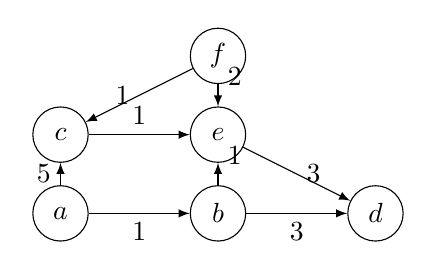
\begin{tikzpicture}[
    vertex/.style={circle,draw,minimum size=20pt,inner sep=0pt},
    >=latex
]
    % Vertices
    \node[vertex] (f) at (2,2) {$f$};
    \node[vertex] (c) at (0,1) {$c$};
    \node[vertex] (e) at (2,1) {$e$};
    \node[vertex] (a) at (0,0) {$a$};
    \node[vertex] (b) at (2,0) {$b$};
    \node[vertex] (d) at (4,0) {$d$};
    
    % Edges with weights
    \draw[->] (f) -- node[above right] {$2$} (e);
    \draw[->] (f) -- node[left] {$1$} (c);
    \draw[->] (c) -- node[above] {$1$} (e);
    \draw[->] (a) -- node[left] {$5$} (c);
    \draw[->] (a) -- node[below] {$1$} (b);
    \draw[->] (b) -- node[below] {$3$} (d);
    \draw[->] (b) -- node[above right] {$1$} (e);
    \draw[->] (e) -- node[right] {$3$} (d);
\end{tikzpicture}
\caption*{Graph for Dijkstra's Algorithm}
\end{figure}

\textbf{Solution:} Let's trace through the first two iterations:

\textbf{Initial State:}
\begin{itemize}[noitemsep]
    \item $a.d = 0$ (source)
    \item All other vertices: $v.d = \infty$
    \item $Q = \{a,b,c,d,e,f\}$
\end{itemize}

\textbf{First Iteration:}
\begin{itemize}[noitemsep]
    \item Extract-Min: vertex $a$ ($d = 0$)
    \item Relax edges from $a$:
        \begin{itemize}[noitemsep]
            \item $(a,b)$: $b.d = \min(\infty, 0 + 1) = 1$
            \item $(a,c)$: $c.d = \min(\infty, 0 + 5) = 5$
        \end{itemize}
    \item $Q = \{b,c,d,e,f\}$
\end{itemize}

\textbf{Second Iteration:}
\begin{itemize}[noitemsep]
    \item Extract-Min: vertex $b$ ($d = 1$)
    \item Relax edges from $b$:
        \begin{itemize}[noitemsep]
            \item $(b,d)$: $d.d = \min(\infty, 1 + 3) = 4$
            \item $(b,e)$: $e.d = \min(\infty, 1 + 1) = 2$
        \end{itemize}
    \item $Q = \{c,d,e,f\}$
\end{itemize}

\textbf{Final Answer:}
\begin{itemize}[noitemsep]
    \item $c.d = 5$ (from first iteration)
    \item $f.d = \infty$ (not yet reached)
    \item $d.d = 4$ (from second iteration)
\end{itemize}

\textbf{Key Insights:}
\begin{itemize}[noitemsep]
    \item Dijkstra's algorithm processes vertices in order of increasing distance
    \item After each iteration, distances are final for the processed vertex
    \item Unreachable vertices maintain distance $\infty$
    \item Each edge relaxation potentially updates the tentative distance to a vertex
\end{itemize}
